% ---
% Este capítulo, apresenta os conceitos sobre o algoritmo genético
% ---

\chapter{Algoritmos Genéticos}
\label{chap:GA}

O algoritmo genético (GA) parte de uma população de \textit{cromossomos} que representam as soluções candidatas para o problema de otimização. Cada uma das soluções é avaliada de acordo com critérios inerentes do problema, para posteriormente serem selecionados e combinados de forma a criar novas soluções candidatas.

Já é possível perceber uma das vantagens do algoritmo, ao fazer uma avaliação direta das soluções de forma paralela. Por exemplo em problemas NP-Completos onde são difíceis de se obter soluções numéricas eficientes, mas é possível testar soluções em tempo polinomial, o algoritmo se torna atrativo. O teste de múltiplas soluções facilita o processamento paralelo aumentando a eficiência do algoritmo.

O algoritmo genético mais simples deverá conter pelo menos uma forma de avaliar os elementos da população, uma forma de seleção baseada nas avaliações e operadores genéticos para gerar a nova população.

\citeauthor{Linden2008} afirma que quanto mais conhecimento especifico sobre o problema for incorporado ao GA, melhor eficiência ele terá. Assim ao definir os operadores que serão utilizados é importante ter em mente que eles devem ser adequados ao problema e não ao contrário.

\section{Codificação dos genes}
Cada cromossomo da população possui uma sequência de genes, que representam os parâmetros para solução do problema. Cada gene terá um possível conjunto de valores, os alelos no equivalente biológico, que para o GA será um alfabeto de valores \( \mathcal{A}\), ou um intervalo caso trabalhando com genes de valores reais. O alfabeto mais simples é o binário com \(\mathcal{A} = \{0, 1\}\), e é muito utilizado pela simplicidade e por ter sido originalmente a escolha de \citeauthor{Holland1992} para explicar os esquemas. Além disso, para ele, os cromossomos de maior comprimento e com menos alelos geravam mais paralelismo intrínseco. Porém essa questão dos esquemas e paralelismo vem levantado questionamentos sobre sua real contribuição para o algoritmo. 

Com o alfabeto binário, os parâmetros são codificados usando sequências binárias, que podem ser representadas por \textit{strings}. Isso envolve conversões dos parâmetros para binário e vice versa. Os operadores de crossover e mutação ficam simplificados ao utilizar esse tipo de codificação. Uma variação da codificação binária é usar o código gray, que evita o chamado abismo de Hamming\footnote{O abismo de Hamming é o efeito que para mudar o valor inteiro em uma unidade na representação binária é necessário alterar todos os bits, por exemplo para ir do número 7 (0111) para o 8 (1000)} 

A representação dos genes em termos gerais deve ser o mais simples e o mais natural possível ao problema. Então é comum usar outras formas de representar os genes, por exemplo, em um problema de escolha da melhor rota é interessante representar os grafos no cromossomo, com isso uma sequência de números inteiros representando cada vértice seria o mais apropriado. Também tem sido muito utilizada a codificação dos genes como números reais, representando assim diretamente os parâmetros do problema, e adaptando então as técnicas de mutação e crossover para se adequar a essa nova codificação. A representação com números reais é muito presente em problemas de otimização para redes neurais, onde o cromossomo é o conjunto de parâmetros de ajuste da rede.

Quando possível é interessante impor na codificação as restrições que são impostas ao conjunto de soluções. Por exemplo, ao utilizar um alfabeto binário para representar valores inteiros, ou reais, pode ser feita a conversão de maneira que os valores máximos e mínimos da representação binária coincidam com os valores permitidos dos parâmetros após a decodificação dos genes. Com isso mais conhecimento é sobre o problema é agregado ao algoritmo melhorando sua resposta. Nem sempre esses limites serão possíveis e será vista outra maneira de impor as condições ao algoritmo através da avaliação.

\section{População, Avaliação e Seleção}
\label{sec:avaliacao}
\subsection{População}
O conjunto de soluções candidatas é definido como a população do algoritmo, que será modificada a cada iteração através dos operadores genéticos. A cada uma dessas populações geradas no instante \(t\) será dado o nome de geração. O tamanho da população é um parâmetro para o algoritmo, e quanto maior, mais soluções serão testadas em paralelo, porém mais recursos computacionais serão usados para cada geração. No algoritmo mais simples, a população é de tamanho fixo e toda substituída na próxima geração, e em outras formas do algoritmo ela pode ter o tamanho variável.

Não existe um número idealizado para o tamanho da população sendo que boa parte dos trabalhos usam 100 como um parâmetro inicial. \citeauthor{Linden2008} indica que um bom começo seria usar \(40 * q\) onde \(q\) é a quantidade de parâmetros codificados em nosso cromossomo, porém para codificações de grafos ou ordenamentos já não seria prático usar esse tipo de escolha para o tamanho da população.

É importante também definir dois conceitos presentes na literatura sobre os GA, que são o \textit{exploitation}\footnote{Exploitation consiste em testar uma região limitada mas promissora do espaço de soluções com a expectativa de melhorar uma solução já conhecida dentro dessa região} e o \textit{exploration}\footnote{Exploration consiste em testar uma região muito mais ampla do espaço de soluções, com a expectativa de encontrar novas soluções promissoras}. O \textit{exploitation} (aproveitamento) é o fato de explorar cada um dos indivíduos da população pelos potenciais resultados que podem gerar através dos descendentes. Já \textit{exploration} (exploração) é o conceito de se manter a diversidade genética da população de forma a explorar o espaço de soluções de forma completa. \citeauthor{Holland1992} indica que deve existir um equilíbrio entre os dois conceitos na população, pois deve-se aproveitar ao máximo cada solução encontrada que poderá gerar novas soluções melhores, e da mesma maneira manter os horizontes sobre o espaço de soluções aberto para a descoberta de novas soluções, evitando a convergência genética.

Defini-se convergência genética como sendo o fato dos cromossomos presentes na população começarem a ficar todos com a codificação similares, levando a entender que o algoritmo atingiu o objetivo, ou pelo menos um máximo ou minimo local. Algumas GAs criam operadores de comparação entre os cromossomos de forma a quantificar essa proximidade como parâmetro para encerramento do algoritmo, mas o mais comum é executar o processo de iteração por \(T\) gerações. A dificuldade de usar a comparação entre os cromossomos está no custo computacional, que dependendo da forma de codificação usada pode ficar muito complexo. \citeauthor{Linden2008} menciona que uma forma de verificar essa convergência é usando o algoritmo de agrupamento K-Means e e depois comparar a distância entre os centróides gerados pelo algoritmo.

Sobre a população podem existir pequenas variações sobre como é evoluída durante o algoritmo. Uma dessas alterações é o \textbf{elitismo}, que separa os \textit{k} melhores indivíduos para sobreviverem na próxima geração. Isso é usado devido ao fato de que os operadores de crossover e mutação poderem destruir esses indivíduos na próxima geração, perdendo assim os bons resultados alcançados. Essa mudança melhora o equilíbrio entre os conceitos de \textit{exploitation} e \textit{exploration} e consequentemente o desempenho do algoritmo, pois mantemos o \textit{exploitation} sobre os \textit{k} indivíduos preservados entre as gerações, e mantemos o \textit{exploration} dando liberdade de escolha arbitrária para os demais \(n-k\) indivíduos da população, onde normalmente \(n \gg k\). 

Outra estratégia para as populações é chamada de \(\mu + \lambda\), onde são criados \(\lambda\) cromossomos gerados por \(\mu\) indivíduos da população atual (geralmente \(\mu < \lambda\)). Feito isso os \(\mu + \lambda\) cromossomos pais e filhos competem para serem selecionados apenas os \(\mu\) melhores indivíduos para formar a nova população. Essa técnica também pode acelerar a convergência genética, devido ao fato da seleção dos melhores que podem apresentar pouca variação genética. Pode ser compensado empregando alguma técnica para manter a diversidade.

Outra alteração possível é denominada \textit{Steady state}, onde em vez de haver a substituição de todos os \textit{n} indivíduos da população anterior para a nova (ou dos \(n - k\) no caso do elitismo) vão sendo criados poucos indivíduos a cada iteração substituindo de forma aleatória os piores pais, isto é, seleciona-se com mais probabilidade os pais com pior avaliação para serem substituídos. Dessa forma existirá uma interação entre cromossomos da geração \textit{t} com as da geração \(t+1\). Um porém de usar essa modificação é de acelerar a convergência genética, pois os indivíduos com pior avaliação sempre serão substituídos de forma rápida, mesmo os recém criados, e também o fato de um cromossomo poder reproduzir com o cromossomo que o gerou, deverá gerar um cromossomo muito parecido com os dois, limitando o \textit{exploitation} desses indivíduos.

Para populações com tamanho variável, basicamente duas técnicas podem ser empregadas. A primeira é determinar um tempo de vida para cada indivíduo baseado em sua avaliação em comparação com a média da população, e a outra técnica é considerar a variabilidade genética. O método que considera a idade dos indivíduos, mantém eles na população por quanto tempo foi determinado na avaliação, e podem levar a condições que a população cresça indefinidamente ou que seja extinta, sendo necessário um controle extra sobre o tamanho da população.

A técnica levando em conta a diversidade, aumenta a população caso perceba-se, através de algum tipo de medição, que os cromossomos da população são semelhantes. Nesse caso alguns cromossomos gerados aleatoriamente podem ser acrescentados a população de modo a manter a exploração do espaço de soluções. Mas como todas as técnicas que devem comparar semelhança entre cromossomos podem ser custosas computacionalmente, pode prejudicar o desempenho desse método.

A população inicial geralmente é iniciada criando cromossomos de forma aleatória, porém pode ser feito de forma a subdividir o espaço de soluções em \textit{n} partes, sendo \textit{n} o tamanho da população, e gerando um cromossomo aleatório para cada uma dessas partes. \cite{Linden2008}.

\subsection{Avaliação}
Para executar uma seleção sobre os cromossomos da população é necessário primeiro existir uma função de avaliação, que deverá fornecer um escalar, de forma a atribuir para cada cromossomo presente na população uma espécie de nota para sua adaptação. O comum nos algoritmos é usar funções de avaliação que são sempre positivas, para o uso no método de seleção da roleta viciada. Alguns cuidados devem ser tomados ao definir a função de avaliação, pois se ela não apresentar variações suficientes para separar os cromossomos que melhor se adaptam dos demais, o algoritmo irá convergir mais lentamente, e se o contrário ocorrer e a função de avaliação tiver valores muito elevados, teremos uma convergência genética rápida demais impedindo a exploração do espaço de soluções podendo ficar restrito a um máximo local.

De uma forma geral consideremos uma função de avaliação \textit{f} e \textit{i} um cromossomo da população. \(f(i) = f_i\) é a avaliação do cromossomo \textit{i}. A probabilidade \(p_i\) de selecionar \textit{i} para reprodução é definida por 

\[p_i = \frac{f_i}{\sum{f}}\]

Onde será adotado que \(\sum{f} = \sum\limits_{j=1}^n {f(j)}\) é a soma das avaliações dos cromossomos da população.

Assim quanto melhor a avaliação de um individuo sobre a média da população, maior é o número esperado de vezes que ele será selecionado. Para evitar que alguns cromossomos, considerados como \textbf{superindivíduos} por \citeauthor{Linden2008}, dominem a próxima geração, devido a uma avaliação muito superior a média dos demais cromossomos, alguns métodos de transformação sobre a função de avaliação podem ser empregados. 

O primeira técnica é a de normalização linear onde pode transformar a função de avaliação na forma \( f' = a * f + b\), onde \textit{a} é normalmente um valor escolhido entre 1 e 2. \citeauthor{Goldberg1989} indica selecionar esses parâmetros de forma que se mantenha o valor médio de \textit{f} e o valor máximo de \textit{f'} seja duas vezes o valor médio. Essa transformação pode gerar problemas pois  dependendo dos valores médio, máximo e mínimo e as escolhas dos coeficientes, a função \(f'\) pode assumir valores negativos que prejudicam a seleção pelo método da roleta viciada que será visto na \autoref{subsec:selecao} sobre seleções. Esse problema pode ser contornado usando outros coeficientes para evitar tal condição passando a se balizar por manter o mínimo de \(f'\) em zero enquanto se mantém o valor médio de \(f'\) igual ao valor médio de \textit{f}.

Outra técnica é o escalonamento Sigma, que procura manter a pressão na seleção constante através das gerações e ao mesmo tempo evitando a convergência genética prematura da população. Assim usando esse método, o valor esperado de vezes que o individuo será selecionado é definido por 
\begin{equation*}
E[i,t] = \left \lbrace  \begin{array}{cc} 1 + \frac{f(i) - \overline{f}(t)}{2\sigma(t)} & \text{, se } \sigma(t) \neq 0 \\
					1.0 & \text{, se } \sigma(t) = 0  \end{array}  \right.
\end{equation*}
onde \(E[i,t]\) é o valor esperado do individuo \textit{i} ser selecionado no instante \textit{t}, \textit{f(i)} é a função de avaliação de \textit{i}, \(\overline{f}(t) = \sum{f}/n\) é a média da função de avaliação dos cromossomos da população no instante \textit{t} e \(\sigma(t)\) é o desvio padrão da função de avaliação dos cromossomos da população no instante \textit{t}. Com essa configuração, mesmo cromossomos que se destaquem demais nas gerações iniciais, devido ao desvio padrão da população ser maior nesse momento, eles não irão dominar a próxima geração, e conforme vai ocorrendo um equilíbrio entre os cromossomos nas gerações futuras e perto da convergência, os que ainda tiverem uma melhor avaliação, serão destacados dos demais para terem maior probabilidade de seleção. Caso o valor esperado se torne negativo para algum individuo, adota-se um valor pequeno como 0.1 permitindo um chance relativamente muito pequena para o individuo se reproduzir. \cite{Mitchell1996}

Em alguns problemas, as restrições sobre o espaço de soluções poderão ser definidas limitando os valores dos parâmetros presentes no cromossomo. Porém em outros casos isso não é possível, principalmente onde, por exemplo, o espaço de soluções não seja convexo. Assim nesses casos é interessante deixar que as soluções sejam avaliadas também fora do espaço de soluções mas aplicar uma penalidade na função de avaliação. Essa penalidade pode ser proporcional ao desvio da solução do espaço permitido, ou uma penalidade constante, o importante é que com a penalidade esse cromossomo seja menos provável de ser selecionado para a próxima geração. O atrativo de permitir esses cromossomos na população, é que mesmo estando fora do domínio do problema, ele pode apresentar um caminho para evolução de soluções melhores, assim se mesmo com a penalidade ele continua com uma boa avaliação, ele deve conter componentes que podem ser aproveitados nos descendentes (\textit{exploitation}).

\subsection{Seleção}
\label{subsec:selecao}

Na etapa de seleção do algoritmo, serão separados os cromossomos para reprodução e consequente geração da próxima população a ser testada. Para tanto o comum é se usar uma componente estocástica para escolha dos pais, e uma determinística que define a probabilidade de escolha de cada pai. A determinística deriva da função de avaliação, que irá definir qual o valor esperado, ou probabilidade de seleção de cada cromossomo presente na população atual. Deve-se levar em consideração de que os métodos apresentados a seguir, podem incorporar o elitismo descrito anteriormente, e selecionar uma quantidade de pais que gere apenas os cromossomos restantes para completar a população.

\begin{description}
	\item[$\bullet$ Roleta Viciada] \text{}
	
O método mais comum e mais simples encontrados no GAs é o da roleta viciada. Nesse método cada cromossomo recebe a probabilidade de ser escolhido definido como \(p_i = f_i / \sum_{j=0}^{n}f_j\), com \(i = 1,2,\dots,n\), sendo \textit{n} o tamanho da população e \textit{f} a função de avaliação. Nesse método que percebe-se a necessidade de \(f > 0\) e a preocupação com cromossomos que tem valores de avaliação destacados perante a média levarem a uma convergência genética precoce. Imagina-se uma roleta que para cada cromossomo é separado uma área proporcional a sua probabilidade de escolha definida pela avaliação, e gira-se a roleta para a seleção de um dos cromossomos. Por exemplo, sendo os valores de avaliação para uma população de 6 cromossomos presentes na \autoref{tab:exemplo_roleta}, obtêm-se a roleta mostrada na Figura~\ref{fig:exemplo_roleta}.

%\begin{minipage}[htb]{\textwidth}
%	\centering
\begin{table}[h!]
	\begin{minipage}[b]{.49\textwidth}
	\centering
		%\begin{table}[htb]
			%\caption{Exemplo avaliação cromossomos}
			%\label{tab:exemplo_roleta}
			\begin{tabular}{l|c|c}
				& f   & p        \\ \hline
				Cromossomo 1 & 152 & 28,84\%  \\
				Cromossomo 2 & 38  & 7,21\%  \\
				Cromossomo 3 & 42  & 7,97\%  \\
				Cromossomo 4 & 5   & 0,95\%   \\
				Cromossomo 5 & 234 & 44,40\%   \\
				Cromossomo 6 & 56  & 10,63\%   \\ \hline
				Total        & 527 & 100,00\%
			\end{tabular}
			\captionof{table}{Exemplo avaliação}
			\label{tab:exemplo_roleta}
		%\end{table}
	\end{minipage}
	\begin{minipage}[b]{.49\textwidth}
	\centering
		%\begin{figure}[ht]
			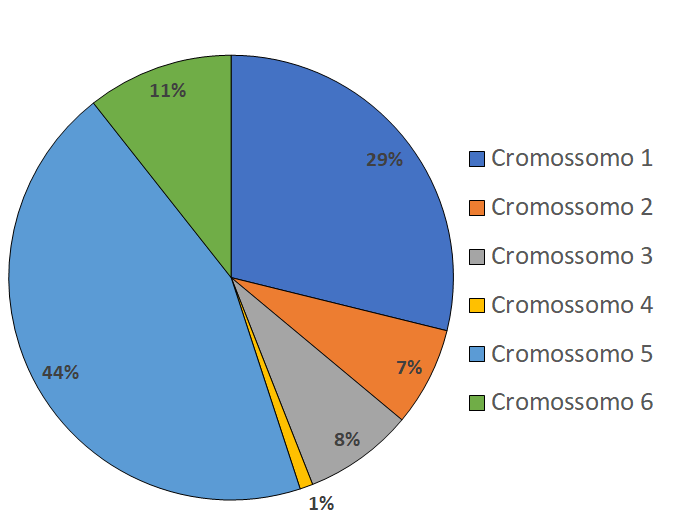
\includegraphics[width=\linewidth]{imagens/exemplo_roleta.png}
			%\caption{Exemplo distribuição em uma roleta viciada}
			\captionof{figure}{Exemplo distribuição em uma roleta viciada}
			\label{fig:exemplo_roleta}
		%\end{figure}
	\end{minipage}
%\end{minipage}
\end{table}

A implementação se torna simples, pois não há necessidade de ordenação dos cromossomos. 

%, e um algoritmo simples para a seleção pode ser visto em \autoref{alg:roleta}, considerando a função \textit{random()} como um gerador de números aleatórios entre 0 e 1. Como pode ser visto, sorteia-se um número entre 0 e o valor da soma das avaliações da população, depois é feito um \textit{loop} iterando pelos valores das avaliações de cada cromossomo e somando a uma variável auxiliar. Ao atingir o valor sorteado, o ultimo individuo que teve seu valor somado a variável auxiliar é retornado.
%
%\begin{algorithm}
%	\LinesNumbered
%	\Entrada{População de cromossomos: populacao}
%	\Saida{Cromossomo selecionado: cromossomo}
%	valor = random() * somaAvaliacao(populacao)\;
%	aux = 0\;
%	i = 1\;
%	\Enqto{aux < valor  {\normalfont \textbf{e}} i <= populacao.tamanho()} {
%			aux = aux + calculaAvaliacao(populacao[i])\;
%			i = i + 1\;
%	}
%	\Retorna{populacao[i-1]}
%	\caption{Roleta viciada}
%	\label{alg:roleta}
%\end{algorithm}

\item[$\bullet$ Amostragem Estocástica Uniforme] \text{}

Uma variação do método da roleta viciada é o Amostragem Estocástica Uniforme (SUS - \textit{Stochastic Universal Sampling}), que em vez de girar a roleta \(w\) vezes, onde \textit{w} define quantos pais deve ser selecionados, é feito apenas um sorteio. O método consiste em alinhar os valores de avaliação dos indivíduos em uma reta contínua, com segmentos proporcionais as avaliações dos cromossomos e normalizados para que a reta tenha tamanho 1. Sorteia-se um número \textit{r} entre 0 e \(1/w\), e depois são gerados \textit{w} ponteiros para reta na forma \(r + j/n \) com \(j = 0, 2, \dots, n-1 \). Os cromossomos são selecionados conforme esses ponteiros caiam sobre seu segmento correspondente na reta e colocados em uma lista. Os cromossomos da lista devem ser embaralhados ou sorteados de forma uniforme sem reposição para dar sequência com os operadores genéticos. Isso é necessário pois como os segmentos são contínuos, os cromossomos que forem selecionados mais de uma vez estarão na sequência na lista. Esse método, diferente da roleta, garante que cada individuo será selecionado para reprodução um número de vezes no intervalo \(\left[ \lfloor E[i,t] \rfloor , \lceil E[i,t] \rceil \right] \), onde \(E[i,t] = \dfrac{f_i}{\sum f} \cdot n\) é o valor esperado de vezes que o cromossomo \textit{i} será escolhido na geração \textit{t}, com \textit{f} sendo a função de avaliação, \(\sum f\) a soma das avaliações dos cromossomos da população no instante \textit{t} e \textit{n} tamanho da população. Importante ressaltar que esse método não impede a questão dos superindivíduos dominarem o processo de seleção podendo levar a convergência genética prematura. 

\item[$\bullet$ Seleção por Torneio] \text{}

Nesse modelo de seleção, são sorteados dois ou mais cromossomos da população com probabilidade uniforme, depois é feito um confronto direto entre os valores de avaliação de cada um, sendo que o que tiver maior valor será o selecionado. Esse mecanismo de seleção evita o favorecimento de indivíduos dominantes da população evitando a convergência genética prematura. Seja \textit{c} a quantidade de cromossomos selecionados para cada rodada do torneio, e \textit{n} o tamanho da população, a probabilidade de seleção de cada um é dada por \(1/n\). Sendo assim a probabilidade de selecionar o pior indivíduo passa a ser \(1/n^c\), pois para ele ser selecionado para a próxima geração deve ser o único na rodada do torneio. Em testes empíricos esse método de seleção apresentou resultados melhores que o da roleta quando \(c=2\), sendo que não é sensível a questões de escalas da função de avaliação e também ao fato da função de avaliação ser negativa. \cite{Linden2008}

\item[$\bullet$ \textit{Ranking}] \text{}

Outro método é a seleção por \textit{ranking}, que também busca prevenir o convergência genética muito rápida, e consiste em ordenar os indivíduos por suas avaliações e depois usar este ranking para definir o valor esperado de cada um, em vez do valor da avaliação. Assim como no método de torneio, não é necessário se preocupar com a escala da função de avaliação. A relação entre os indivíduos \textit{i} e o \(i+1\) será a mesma independente dos valores avaliados para cada um. 

Cada cromossomo é classificado com os valores de 1 a \textit{n}, definido como \textit{rank}, indo do pior avaliado para o melhor. O valor esperado de cada cromossomo será dado por \[E[i,t] = \min + (\max - \min) \frac{rank(i,t) - 1}{n - 1} \] onde \(\max\) é o valor esperado para o melhor indivíduo e \(\min\) para o pior. Como há as restrições de \(\max \geq 0\) e \(\sum_i E[i,t] = n\), pois deve-se manter a população, é necessário então que \(1 \leq \max \leq 2\) e \(\min = 2 - \max\).

O valor proposto por Baker é \(\max = 1,1\), e esse método tem a desvantagem de diminuir a pressão seletiva, o que pode levar ao GA uma convergência mais lenta, porém mantém a diversidade garantindo uma melhor exploração do espaço de soluções. Uma forma de manter a pressão seria usar uma função exponencial para definir os valores esperados de cada cromossomo. Seja qual for a forma de mapeamento dos valores esperados, depois pode ser utilizado o método SUS ou da roleta viciada para selecionar os pais da próxima geração.\cite{Mitchell1996}


\item[$\bullet$ Seleção Boltzmann] \text{}

Esse método é inspirado no \textit{simulated annealing}, onde variando a temperatura de forma continua, pode-se controlar a taxa de seleção. O algoritmo inicia com uma temperatura alta, garantindo que todos na população tem maior probabilidade de reprodução, reduzindo a pressão seletiva, e conforme as iterações do algoritmo são executadas, a temperatura é reduzida gradativamente, aumentando assim a pressão seletiva, e restringindo para apenas os melhores continuarem a se reproduzirem. Uma implementação tipica do modelo é \[ E[i,t] = \frac{e^{f_i/\mathcal{T}}}{\frac{\sum_j e^{f_j/\mathcal{T}}}{n}}\] onde \(\mathcal{T}\) representa a temperatura, e \textit{n} o tamanho da população, assim no denominador da expressão é representada a média da avaliação da população no instante \textit{t}. \cite{Mitchell1996}

\end{description}

\section{Operadores genéticos}

Definidos como serão a população e a codificação dos cromossomos, além dos métodos de avaliação e seleção do GA, deve-se agora selecionar quais operadores genéticos serão usados. Para cada operador há um parâmetro associado que define uma probabilidade de uso do operador a cada etapa do algoritmo, e os operadores podem ser combinados. Os parâmetros podem ser fixos ou variarem conforme a evolução do algoritmo. Lembrando que com o uso do elitismo, teremos indivíduos que passarão para a próxima geração sem modificação pelos operadores genéticos.

\subsection{Crossover}
O operador mais característico e diferencial do algoritmo genético é o de crossover ou recombinação. É com esse operador que dois cromossomos tem suas características combinadas gerando um novo indivíduo que potencialmente terá avaliação melhor que seus pais. Associado a esse operador existe um parâmetro, \(p_c\), que determina a probabilidade de ser executado o crossover sobre um par de cromossomos selecionados. Esse parâmetro, tem valor normalmente alto entre 0,8 e 1, e se após o sorteio ficar definido que não será usado o operador, um dos pais é passado sem alterações para as próximas etapas.

\begin{description}
\item[$\bullet$ Crossover de um ponto] \text{}

Esse é o operador mais simples de crossover, onde é sorteado um ponto de corte dentro do cromossomo para ocorrer a ``quebra'' da sequência dos genes. O cromossomo é formado por uma sequência \textit{l} de genes, e entre esses genes há \(l-1\) pontos de corte que definem as posições onde o cromossomo poderá ser interrompido para ser combinado com a outra parte do outro cromossomo. Após a seleção de dois pais, é feito um sorteio uniforme para o ponto de corte. Podem ser gerados dois novos cromossomos, sendo o primeiro combinando o material genético do pai A a esquerda do ponto de corte e o material genético do pai B a direita do ponto, e o segundo com o inverso. Algumas implementações aproveitam os dois novos indivíduos para a nova geração, outros ainda realizam um sorteio com igual probabilidade de escolha para um dos dois novos cromossomos.

\begin{figure}[ht]
	\centering
	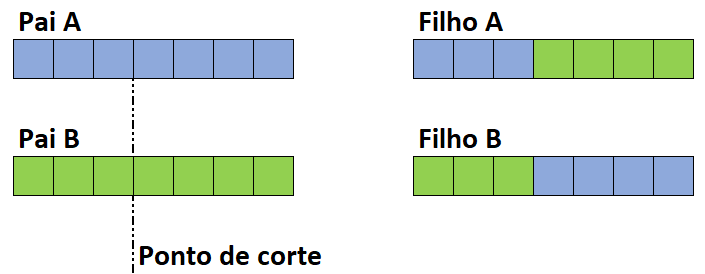
\includegraphics[width=0.75\linewidth]{imagens/exemplo_cross_1pto.png}
	\caption{Crossover com um ponto}
	\label{fig:ex_cross_1pto}
\end{figure}

Existem dois detalhes sobre o crossover de um ponto, primeiro se uma boa solução do problema estiver codificado nos genes extremos do cromossomo, a chance de manter esse dois genes no novo indivíduo reduz muito, pois o novo elemento da população terá a parte inicial do cromossomo ou a parte final somente. Isso também leva ao segundo problema, pois existem uma certa ``preferência'' no método para determinadas posições do cromossomo, já que as partes trocadas entre os pais sempre contém os extremos. \cite{Mitchell1996}.

\item[$\bullet$ Crossover de dois ou mais pontos] \text{}

Para melhorar as questões levantadas pelo crossover de um ponto, surgiram as derivações para terem mais pontos de corte no operador. O processo se mantém o mesmo, no entanto em vez de sortear um ponto de corte para executar as trocas de material genético, são sorteados dois ou mais pontos, e os cromossomos pais tem então suas sequências de genes intercaladas entre esses pontos de corte. Um exemplo para dois pontos é apresentado na \autoref{fig:ex_cross_2pto}.

\begin{figure}[ht]
	\centering
	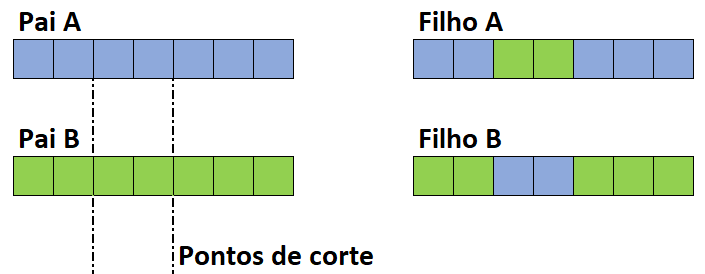
\includegraphics[width=0.75\linewidth]{imagens/exemplo_cross_2ptos.png}
	\caption{Crossover com dois ponto}
	\label{fig:ex_cross_2pto}
\end{figure}

Fazendo o crossover em  mais pontos diminuí os problemas encontrados quando utilizado apenas um ponto de corte. Aumenta-se a chance de manter os genes que estejam em locus distantes na sequência do cromossomo que contribuem para boa avaliação do indivíduo, e diminui-se um pouco o detalhe de uso dos extremos, pois pode-se combinar apenas a parte central de um dos pais.

\item[$\bullet$ Crossover uniforme] \text{}

Esse operador é capaz de combinar qualquer esquema presente nos cromossomos. O conceito de esquemas será melhor explorado na \autoref{sec:esquemas}, mas para o entendimento do crossover, o esquema pode ser considerado como uma máscara para os genes do cromossomo, fixando alguns desses genes e deixando outros livres. Considerando que os genes fixos no esquema são os responsáveis pela boa avaliação do cromossomo, dependendo da distância nas posições deles, foi visto que os operadores de crossover usando pontos de cortes podem interromper mais facilmente esses esquemas. Com o crossover uniforme esse efeito é minimizado, permitindo que todos os esquemas tenha probabilidade iguais de serem transmitidos aos filhos. O exemplo simplificado do operador pode ser visto em \autoref{fig:ex_cross_unif}
	
	\begin{figure}[ht]
		\centering
		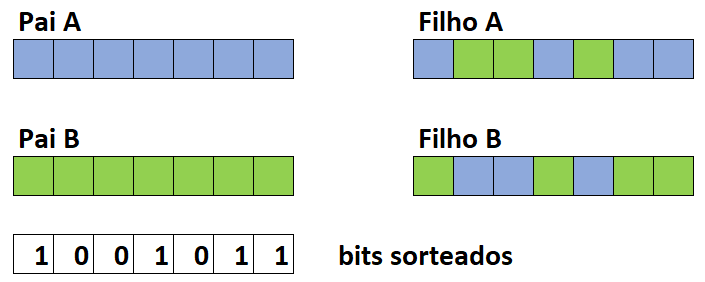
\includegraphics[width=0.75\linewidth]{imagens/exemplo_cross_uniforme.png}
		\caption{Crossover uniforme}
		\label{fig:ex_cross_unif}
	\end{figure}

A diferença com relação aos operadores de combinação anteriores se deve ao fato de que é feito um sorteio dos valores 1 ou 0 com iguais probabilidades para cada posição do cromossomo criando uma sequência binária. Utiliza-se então o resultado do sorteio para definir se será usado o gene do pai A ou do B. Como todas as sequências tem iguais probabilidades de ocorrerem, justifica-se o fato de que os esquemas passam a ter a mesma probabilidade de se manterem durante a reprodução.

\citeauthor{Mitchell1996} menciona uma outra forma de realizar o operador de crossover uniforme, onde seguindo o mesmo raciocínio dos pontos de cortes, se realiza um primeiro sorteio para decidir por qual pai começa a construção do filho, e para cada posição do gene é feito um novo sorteio com igual probabilidade para decidir se continua copiando a sequência do pai atual ou se passa a copiar do outro pai, alcançando os mesmos resultados do procedimento descrito anteriormente.

\item[$\bullet$ Crossover baseado em maioria] \text{}

O ultimo operador de crossover apresentado será um que combina vários pais simultaneamente, e não é muito utilizado pois pode levar a convergência genética muito rápida. O conceito por trás desse operador é selecionar \textit{z} pais com \(3 \le z \le n\), sendo \textit{n} tamanho da população, e depois definir para cada gene o valor correspondente a maioria. Alternativamente pode ser feito de forma a calcular uma distribuição para cada gene baseado nos valores encontrados no \textit{z} cromossomos, e depois realizando uma seleção nos moldes da roleta viciada para decidir qual gene utilizar. Esse crossover acaba gerando mais um parâmetro para o algoritmo, pois é necessário definir qual o valor de \textit{z}
 
\end{description}

Os operadores descritos podem em geral serem usados com qualquer tipo de codificação, em especial com codificações binárias seu uso são imediatos. Para algumas outras codificações ajustes são necessários. Para representações com reais paras os genes, ou de grafos como na programação genética, os operadores de crossover que usam pontos de corte ou o uniforme funcionam normalmente, pois definido os pontos de corte basta executar os intercâmbios dos valores situados entre eles. 

Para cromossomos baseados em ordem, isto é, a ordem da sequência apresentada no cromossomo representa o fenótipo do indivíduo e consequentemente sua avaliação, usar o crossover de um ponto ou mais pode gerar um problema. Como o operador se baseia na posição dos genes para fazer a concatenação, e nesse tipo de cromossomo as posições dos genes mudam, é necessário adaptar o operador. A forma mais simples de realizar essa adaptação é, em vez de intercambiar diretamente os valores entre os pontos de corte, mantém-se os valores de um dos pais selecionado, mas utiliza-se a ordem para esses valores encontradas no segundo pai. Por exemplo na \autoref{fig:ex_cross_ordem}, podemos ver que o pai A possui na região entre os dois pontos de corte a ordem 7 - 1, e esses mesmos valores estão na ordem 1 - 7 no pai B, assim o operador muda a ordem dos valores nesse pedaço para ficar com a mesma ordem do pai B e o resultado é visto no filho A. No filho B o inverso ocorre, sendo que na região de corte é usada a ordem que os valores aparecem no pai A. Pode ser feita uma adaptação análoga para o crossover uniforme. Para o operador baseado em maioria, pode ser feito inciando o primeiro item da sequência pela maioria presente nos pais selecionados, e nas demais posições ir pela maioria encontrada nos pais que seguem o gene escolhido anteriormente.

\begin{figure}[ht]
	\centering
	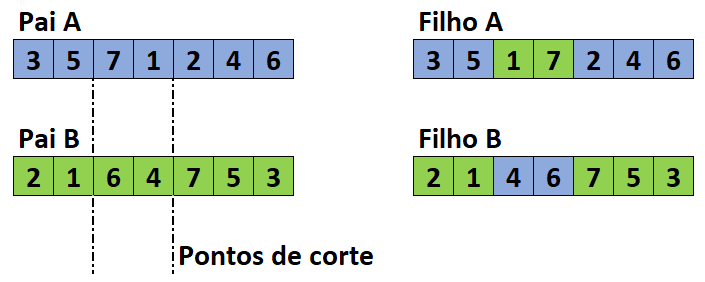
\includegraphics[width=0.75\linewidth]{imagens/exemplo_cross_ordem.png}
	\caption{Crossover com codificação por ordem}
	\label{fig:ex_cross_ordem}
\end{figure}

Quando a codificação for baseada em números reais, o operador de crossover pode ser modificado para em vez de escolher um dos dois valores do gene presentes nos pais, considerar um deles como mínimo e o outro como máximo e realizar um sorteio uniforme no intervalo para o valor do gene. Isso irá gerar filhos bem distintos dos pais, aumentando o aspecto de \textit{exploration} do algoritmo.

\subsection{Mutação}
O operador de mutação é responsável em aumentar o aspecto de \textit{exploration} do GA, e através dele que é possível explorar novas soluções ainda não testadas. Existe um parâmetro, \(p_m\) associado a esse operador referente a taxa de mutações presentes no algoritmo, sendo que essa taxa usada é um valor baixo na ordem de 0,5\% para menos. A taxa deve ser baixa, pois quanto maior for, mais o algoritmo irá se assemelhar a uma busca randômica. Mantendo as probabilidades de mutação baixa garante apenas que novas soluções serão apresentadas quando o algoritmo já estiver convergindo, e assim representa uma alternativa caso o GA estiver convergindo para um máximo local.

O procedimento é simples, para cada gene é feito um sorteio com a probabilidade determinada para a taxa de mutação, caso o sorteio tenha um resultado positivo, o gene em questão será modificado. Essa modificação depende do tipo de codificação que foi utilizado. Para codificação binária há duas opções, inverte-se o estado do bit que deve sofrer a mutação, ou pode-se sortear um novo bit com probabilidade igual para 0 ou 1. Usando essa segunda forma, a taxa de mutação resultante será \(p_m \cdot 0,5\), onde \(p_m\) é o parâmetro de mutação escolhido.

Sobre a codificação binária, existe um detalhe sobre o operador mutação. Como cada bit tem uma significância para o parâmetro que representa do problema, dependendo do bit que for modificado pode representar ``saltos'' maiores ou menores no espaço de soluções e consequentemente nos valores da avaliação. Uma forma de contornar esse dilema, seria definir \(p_m\) proporcional à significância do bit que será modificado. Outra forma seria primeiro transformar a representação binária na variável do problema, realizar uma mutação sobre esse valor, e depois transformar de volta a variável para binário.

Para codificações em inteiros ou em reais, a mutação será na forma de um sorteio sobre o valor do gene. Esse pode usar alguma distribuição conhecida para toda a faixa dos valores que a variável pode assumir, ou usar uma distribuição normal para definir um valor de desvio para a variável e condicionando o resultado para ficar nos limites ou, como visto anteriormente na \autoref{sec:avaliacao}, permitir esse valores fora das restrições que serão penalizados pela função de avaliação.

As mutações para codificações que usam ordem podem ser feita de duas formas. A primeira se um gene deverá ser modificado, sorteia-se outro gene aleatoriamente e é feita a permutação dos dois. Na segunda forma defini-se dois pontos no cromossomo e é feita ou uma mistura dos elementos entre esses dois pontos, ou inverte-se a ordem entre esses dois pontos.

Para cromossomos baseados em grafos, ou árvores, a sugestão é remover o ramo selecionada para mutação, e gerar um novo aleatório, seguindo o mesmo processos usado para gerar a população inicial.

É comum usar para o parâmetro de taxa de mutação, um valor variável, que pode ir aumentando a cada iteração do algoritmo, permitindo assim que conforme vai se atingindo a convergência genética, o GA não perca sua característica de \textit{exploration}, buscando soluções totalmente novas.

\subsection{Outros operadores}
Existem outros operadores menos usados no algoritmo como por exemplo o de inversão proposto por Holland e alguns que operam sobre como são formados os pares para reprodução.

\citeauthor{Holland1992} propôs um operador que inverte parte da sequência do cromossomo, pois percebeu a questão do crossover de um ponto de ter uma maior probabilidade em interromper esquemas com genes mais afastados na sequência. Esse operador é inspirado pelo que acontece na genética real, onde a função do gene não depende da sua posição, portanto invertendo parte do cromossomo, sua essência seria mantida. Para adaptar esse operador no GA, além do valor do gene, o cromossomo deve armazenar qual a sua posição original também, o que acarreta uma maior custo computacional. O funcionamento básico do operador é selecionar dois pontos aleatórios no cromossomo, e inverter a ordem dos genes encontrados nesse intervalo. Quando foi realizar o crossover, como os pais selecionados podem ter a ordem dos genes alteradas, utiliza-se um deles como referência e ordena-se o segundo da mesma forma, assim o crossover não correrá o risco de repetir genes na concatenação das partes. Testes com inversão foram feitos mas nenhum obteve resultados indicando que o uso desse operador melhora o desempenho do GA. \cite{Mitchell1996}.

Além desse operador, foram feitos alguns experimentos com operadores de seleção que procuram determinar outros fatores na seleção dos pais, como por exemplo não selecionar dois indivíduos que tenham o genótipo parecido, evitando assim convergência genética prematura e buscando que a combinação entre pais geram filhos diferentes dos encontrados na população até o momento.

Também existem as versões dos operadores apresentados para cromossomos diplóides, onde o genótipo possui um par de cromossomos, sendo que deve ser utilizado o aspecto de dominância dos alelos para definir o fenótipo. A maior diferença está no operador de crossover, pois por serem indivíduos diplóides, ocorre primeiro a separação do par de cromossomos em gametas, feito o crossover e depois recombinação entre os gametas dos pais selecionados. Em \citeonline{Goldberg1989} é possível verificar uma análise mais detalhada sobre esse assunto.

\section{Fundamentos teóricos}
\subsection{Esquemas}
\label{sec:esquemas}
O conceito de esquema (\textit{schema} ou \textit{schemata}) foi primeiro definido por \citeauthor{Holland1992}, em uma tentativa de especificar por qual razão o algoritmo genético funciona e pode ser eficiente. Foi apresentado também por \citeauthor{Goldberg1989} como teorema fundamental do GA, e ficou conhecido por Teorema dos Esquemas (\textit{Schema Theorem}). Por trás desse conceito, Holland ainda explica a teoria do paralelismo implícito presente no algoritmo razão da qual ele apresentar certa eficiência se comparado a outros algoritmos.

Para explicar o conceito primeiro define-se que o cromossomo é uma sequência, de comprimento \textit{l}, de genes que podem ter os valores presentes no alfabeto \(\mathcal{A}\). Para simplificar as definições e cálculos e sem perda de generalidade, foi escolhido um alfabeto binário \(\mathcal{A} = \{0, 1\}\) e os cromossomos são portanto sequências binárias. 

Define-se o esquema, \textit{H}, como uma sequência de tamanho \textit{l}, e que pode ter os valores contidos em \(\mathcal{A}^+ = \{0, 1 , *\}\), sendo \textit{*} considerado um valor coringa e representa uma posição no cromossomo que não importa (\textit{don't care}). É possível definir um esquema para qualquer alfabeto, apenas acrescentando o caractere coringa ao alfabeto gerador dos cromossomos. O esquema funciona como um gabarito ou \textit{template} e existirão subconjuntos de cromossomos que se encaixam nesse gabarito. 

Define-se instância como cada cromossomo que se enquadra em determinado esquema.

Por exemplo, supondo uma população de cromossomos com comprimento \(l=8\), o esquema \mbox{\(H=**11*0*1\)} tem os cromossomos \(A_1=00110001\) e \(A_2=10111011\) como instâncias. Assim seja \(\mathcal{C}_l\) o conjunto de todos possíveis cromossomos binários de comprimento \textit{l}, e \(\mathcal{E}_l\) o conjunto de todos possíveis esquemas de comprimento \textit{l}, então \(\mathcal{C}_l \subset \mathcal{E}_l \) e temos \(2^l = |\mathcal{C}_l|\) possíveis cromossomos e \(3^l = |\mathcal{E}_l|\) possíveis esquemas.

Define-se \textbf{ordem} do esquema \textit{H}, denotada por \(o(H)\), como quantas posições possuem valor fixo no esquemas, isto é, quantas posições no esquema são diferentes de \textit{*}. No exemplo anterior \(H=**11*0*1\) possui ordem 4, \(o(**11*0*1) = 4\).

Define-se \textbf{tamanho} do esquema \textit{H} (\textit{defining length}), denotado por \(\delta(H)\), como a diferença entre as posições do ultimo valor definido no esquema e do primeiro definido. Por exemplo para o esquema \(H=**11*0*1\) seu tamanho é 5, pois o ultimo valor definido está na posição 8 e o primeiro na posição 3, \(\delta(**11*0*1) = 5\). 

Goldberg usou o simbolo \textit{H} pois o esquema define um hiperplano do espaço de dimensão \textit{l} que representa as sequências binárias de comprimento \textit{l}. Considerando sequências binárias e esquemas de comprimento \(l=3\), é possível desenhar a representação dos hiperplanos de forma geométrica, que pode ser visto na \autoref{fig:schema_hyperplane}. Os vértices são esquemas de ordem 3, as linhas de ordem 2 e os planos de ordem 1.

\begin{figure}[h!]
	\centering
	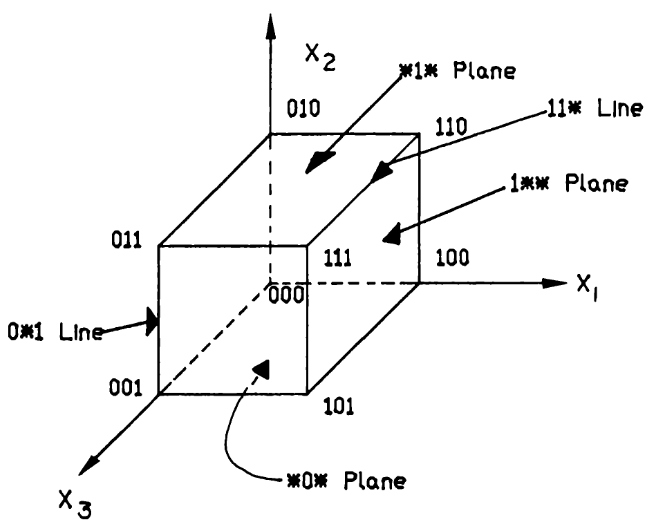
\includegraphics[width=0.75\linewidth]{imagens/schema_hyperplane.png}
	\caption{Representação dos esquemas como hiperplanos em um espaço tridimensional. \cite{Goldberg1989}}
	\label{fig:schema_hyperplane}
\end{figure}

Dessas definições, pode ser verificado que quanto maior for o tamanho de um esquema \(\delta(H)\), maior será sua probabilidade de ser desfeito com os operadores genéticos de crossover, e quanto maior sua ordem \(o(H)\), maior será a probabilidade do operador de mutação de destruí-lo. Contudo, deve-se manter em mente que esses mesmos operadores aplicados aos melhores cromossomos avaliados e selecionados, também podem produzir cromossomos com avaliação ainda melhor.
%Apesar da probabilidade de modificar alguns dos esquemas presentes e que foram bem avaliados, pois os operadores serão aplicados aos cromossomos selecionados e portanto que possuem melhor avaliação me média, existe a chance de com isso encontrar esquemas que responderão melhor ainda para o problema em questão. 

Como esquemas de ordem e tamanho maiores estão mais sujeitos a serem destruídos, os esquemas mais curtos e que mais contribuem para a avaliação dos cromossomos, tendem a ser preservados, e esses constituem os blocos de construção (\textit{building blocks}) citados por \citeauthor{Goldberg1989}.

O que \citeauthor{Holland1992} indica como \textbf{paralelismo intrínseco} se atribui ao fato, de que apesar do algoritmo estar avaliando \textit{n} indivíduos contidos na população da geração presente, ele está também avaliando de forma implícita um número bem maior de esquemas. Qualquer sequência binária de comprimento \textit{l} é uma instância de \(2^l\) esquemas. Por exemplo a sequência 11, é uma instância dos seguintes esquemas: **, 1*, *1 e 11. Estendendo para a população de tamanho \textit{n} existem portanto um total de até \(n \cdot 2^l\) esquemas, assim o total de esquemas em determinada população será um valor entre \(2^l\), caso todos os cromossomos sejam iguais, e \(n \cdot 2^l\), caso todos diferentes. Por essa razão o GA avalia uma quantidade de esquemas maior do que a quantidade de indivíduos presentes na população.

\subsection{Teorema fundamental do GA}
A \autoref{eq:schema_theorem} define o Teorema dos Esquemas proposto por \citeauthor{Holland1992} e que pode ser visto também em \citeonline{Goldberg1989}.

\begin{equation}
E[m(H,t+1)] \ge \frac{\hat{u}(H,t)}{\overline{f}(t)} m(H,t)\left( 1 - p_c \frac{\delta(H)}{l - 1} \right) \left[(1 - p_m)^{o(H)} \right]
\label{eq:schema_theorem}
\end{equation}

A equação define que o valor esperado da quantidade de esquemas presentes na próxima população baseado em sua avaliação comparada com a média, as probabilidades de crossover e mutação associadas aos seus tamanho \(\delta(H)\) e ordem \(o(H)\).

O teorema pode ser verificado através da estimação do aumento ou diminuição das instâncias dos esquemas presentes na população. Consideremos uma população \(\theta\) de tamanho \textit{n} de cromossomos com codificação binária e comprimento \textit{l}. Seja \textit{H} um esquema que tenha ao menos uma instância na população na geração \textit{t}. Defini-se \(M(H)\) o conjunto de todos os cromossomos que são instâncias de \textit{H} e \(M(H, t) \subseteq M(H)\) o conjunto dos cromossomos que são instâncias de \textit{H} na população no instante \textit{t}. Temos \(m(H, t) = |M(H,t)|\) definido como o número de instâncias de \textit{H} no instante \textit{t} presentes na população. 

Definimos 
\[\hat{u}(H,t) = \frac{\sum\limits_{i \in M(H,t)}f(i)}{m(H,t)}\]
onde \textit{i} é um cromossomo na população que é instância de \textit{H}, e \(f(i)\) é a função de avaliação. Assim \(\hat{u}(H,t)\) é a média das avaliações das instâncias de \textit{H} no instante \textit{t}.

Relembrando que a probabilidade de um indivíduo ser escolhido para seleção com o método da roleta viciada é definido por \(p_i = f(i) / \sum_{j \in \theta}{f(j)}\), com \(i = 1,2,\dots,n\). Sendo \(\eta(i,t)\) a quantidade de vezes que o cromossomo \textit{i} é selecionado na população no instante \textit{t}, o valor esperado de \(\eta\) será \(E[\eta(i,t)] = n \cdot p_i\). Se \(\overline{f}(t) = \sum_{j \in \theta} {f(j)} / n\) é a média das avaliações dos cromossomos da população no instante \textit{t}, o valor esperado de \(\eta(i,t)\) pode ser expresso como \(E[\eta(i,t)] = f(i) / \overline{f}(t)\)

O valor esperado da quantidade de instâncias de \textit{H} em \(t+1\) considerando \textbf{apenas a seleção} descrita e sem usar os operadores de crossover e mutação será dado por:
\begin{align}
	E[m(H,t+1)] &= \frac{\sum\limits_{i \in M(H,t)} {f(i)}}{\overline{f}(t)} \nonumber \\
				&= \frac{\hat{u}(H,t)}{\overline{f}(t)} m(H,t)
\label{eq:valor_esperado_H}
\end{align}

Assim é verificado que a quantidade esperada de instâncias do esquema \textit{H} na próxima geração depende diretamente da média das avaliações das instâncias do esquema na geração atual e pode ser concluído que esquemas com avaliação maior que a média irão aumentar ao passo que os com avaliação menor diminuirão.

Como visto antes, os operadores de crossover e mutação podem tanto construir como destruir as instâncias do esquema \textit{H}, e que a probabilidade de destruir é proporcional as características do esquema dado pela ordem \(o(H)\) e pelo tamanho \(\delta(H)\). 

Considerando apenas o fato destrutivo dos operadores, para o caso do crossover de ponto único, a probabilidade de um esquema ser destruído é definida por \(D_c(H) = {\delta(H)}/{l - 1}\). Sendo \(p_c\) a probabilidade do operador ser aplicado, então o limite inferior da probabilidade de sobrevivência do esquema, \(S_c(H)\), pode ser estimado como:
\begin{equation}
S_c(H) \ge 1 - p_c \frac{\delta(H)}{l - 1} % parte depois do 1 - é o limite superior da probabilidade de destruir ele, e 1 - p_destroy e a probabilidade de sobreviver%
\label{eq:survive_cross}
\end{equation}
e pela equação é verificado que quanto menor o tamanho do esquema, maior sua probabilidade de sobrevivência. Esse é um limite inferior pois se por exemplo dois cromossomos selecionados para o crossover forem idênticos, mesmo que o ponto de corte do operador seja dentro dos limites do esquema, essa instância não será destruída.

Já para o operador de mutação, considerando \(p_m\) como a probabilidade de um bit sofrer mutação, a probabilidade de sobrevivência do esquema a esse operador, \(S_m(H)\), é dada por:
\begin{equation}
S_m(H) = (1 - p_m)^{o(H)}
\label{eq:survive_mut}
\end{equation}
e novamente quanto menor a ordem do esquema, maior probabilidade de sobrevivência.

Assim, a \autoref{eq:valor_esperado_H}, pode ser modificada combinando com as Equações \ref{eq:survive_cross} e \ref{eq:survive_mut}, obtendo então a \autoref{eq:schema_theorem} do teorema fundamental.

Em palavras o teorema pode ser interpretado como: "o GA tende a preservar com o decorrer do tempo aqueles esquemas com maior avaliação média e com menores ordem e tamanho, combinando-os como blocos de construir de forma a buscar a melhor solução". \cite{Linden2008} 
 
%\subsection{Two-armed bandit}
%\citeauthor{Holland1992} menciona que a adaptação possui uma tensão entre os componentes de \textit{exploitation} e \textit{exploration}, e que a análise de esquemas demonstrava, assumindo certas condições, que o GA atingi um certo equilíbrio próximo do ótimo. A permutação entre os dois podem ser comparados com o \textit{``Two-armed bandit problem''}\footnote{Uma máquina caça-níquel é também conhecida como \textit{One-armed bandit}}.\cite{Mitchell1996}
%
%O problema é descrito como um jogador com \textit{N} moedas e uma máquina caça-níquel com duas alavancas, sendo que uma delas(\(A_1\)) paga com média \(\mu_1\) e desvio-padrão \(\sigma_1\) e a outra(\(A_2\)) paga com média \(\mu_2\) e desvio-padrão \(\sigma_2\). Esses valores não variam, são independentes e são desconhecidos ao jogador. O objetivo do jogador é maximizar os lucros, porém como não tem informações sobre qual das alavancas paga mais, só pode estimar realizando jogadas nas duas. 
%
%\citeauthor{Mitchell1996} descreve uma solução simples para o problema seguindo o que foi proposto por \citeauthor{Holland1992} e que pode ser visto em detalhes em \citeonline{Holland1992}. Considerando sem perda de generalidade que \(\mu_1 > \mu_2\), ou seja, a alavanca \(A_1\) paga mais que a \(A_2\), e sendo \(A_h(N, N-n)\) e \(A_l(N,n)\) as alavancas com maior e menor valores pagos observados respectivamente, após \textit{N} tentativas, sendo \(N-n\) tentativas usadas em \(A_h\) e \textit{n} tentativas na \(A_l\). O que se busca é o valor \(n = n^*\) que maximize o lucro. A melhor estratégia seria colocar as \textit{N} apostas na alavanca que paga mais, porém como ela não é conhecida isso não é possível.
%
%Duas possibilidades podem ocorrer, ou \(A_l\) corresponde a pior alavanca e nesse caso houve prejuízo somente nas \(n\) apostas feitas em \(A_l\) (as perdas dadas por \((N-n)(\mu_1-\mu_2)\)), ou \(A_l\) corresponde a melhor alavanca e então houve prejuízo nas \(N- n\) apostas colocadas em \(A_h\) (perdas dadas por \(n(\mu_1-\mu_2)\)). Seja \textit{q} a probabilidade de \(A_l\) ser na verdade a melhor alavanca \(A_1\), isto é, \(q = P(A_l(N,n) = A_1)\), assim as perdas \(L(N-n,n)\) após \textit{N} tentativas é dado por:
%
%\begin{equation*}
%L(N-n,n) = q(N-n)(\mu_1-\mu_2) + (1-q)n(\mu_1-\mu_2)
%\end{equation*}
%
%Como o desejado é \(n = n^*\) que minimiza essa função (ou seja maximiza o lucro), tomando a derivada com relação a \textit{n} e igualando a zero.
%\begin{equation*}
%\frac{dL}{dn} = (\mu_1-\mu_2)\left( 1 - 2q + (N-2n)\frac{dq}{dn}\right) = 0
%\end{equation*}
%
%Que para ter uma solução é necessário expressar \textit{q} em função de \textit{n}. Sejam \(S_1^n\) a soma recebida pelas apostas em \(A_1\) e \(S_2^{N-n}\) a soma recebida pelas apostas em \(A_2\). Então \textit{q} pode ser expresso na forma:
%
%\begin{align}
%q 	&= P\left(\frac{S_2^{N-n}}{N-m} > \frac{S_1^n}{n}\right) \nonumber \\
%	&= P\left( \left( \frac{S_2^{N-n}}{N-m} - \frac{S_1^n}{n} \right) < 0 \right)
%\label{eq:prob_q}
%\end{align}
%
%que indica de fato a probabilidade de observar que \(A_2\) pagou mais que \(A_1\). Como \(S_1^n\) e \(S_2^{N-n}\) são variáveis aleatórias, sua diferença também é uma v.a. e a probabilidade descrita em \autoref{eq:prob_q} é a área abaixo da curva de distribuição na parte menor que zero. \citeauthor{Holland1992} aproximou essa probabilidade usando o teorema central do limite assumindo a distribuição normal. Na segunda edição, Holland atribui a correção dessa aproximação para Dan Frantz, que usou a teoria dos grandes desvios(\textit{theory of large deviations}), para aproximar essa probabilidade e chegar ao resultado:
%
%\begin{equation*}
%n^* \approx c_1 ln\left( \frac{c_2 N^2}{ln(c_3 N^2)} \right)
%\end{equation*}
%
%onde \(c_1\), \(c_2\) e \(c_3\) são constantes positivas. Rearranjando os termos obtêm-se:
%
%\begin{equation*}
%N - n^* \approx e^{n^*/2c_1} \sqrt{\frac{ln(c_3 N^2)}{c_2}} - n^*
%\end{equation*}
%
%Conforme \(n^*\) aumenta, o termo exponencial domina a equação, e pode-se aproximar mais ainda obtendo:
%
%\begin{equation*}
%N - n^* \approx e^{cn^*}
%\end{equation*}
%
%que indica em resumo que o valor ótimo de apostas \(N-n^*\) feitas à melhor alavanca observada deve aumentar exponencialmente conforme o número de apostas feitas na pior alavanca observada. \cite{Mitchell1996}
%
%O que o Teorema dos Esquemas sugere é que da mesma forma que o problema descrito \textit{``two-armed bandit''} que pode ser estendido a um problema com \textit{k} alavancas(\textit{``k-armed bandit''}), o GA aumenta de forma exponencial as tentativas feitas com os melhores esquemas observados com relação as tentativas feitas aos piores esquemas. \citeauthor{Goldberg1989} indica que na verdade o GA deve ser comparado a uma composição de \textit{k-armed bandits}.
%
%\citeauthor{Mitchell1996} faz uma ressalva com a comparação com relação ao fato de que no caso do \textit{two-armed bandit}, as alavancas são independentes, que não é o caso do GA, pois os esquemas interagem entre eles, pois por exemplo, o valor observado de retorno do esquema \(111*\ldots*\) tem influência sobre o valor observado do retorno de \(1***\ldots*\).
%
%\subsection{O GA como uma cadeia de Markov}
%O teorema dos esquemas versa sobre a evolução dos esquemas presentes no algoritmo, porém para tentar determinar exatamente fatores como a distribuição da população, das avaliações e da convergência do algoritmo conforme as iterações, foram procurados outros modelos matemáticos para determinar o comportamento do GA. Um desses modelos descritos por \citeauthor{Nix1992}, modela o GA na forma de uma cadeia de Markov, para uma população finita. Assim o estado atual é definido pela presente população, que através de uma matriz de transição \textit{Q} define a probabilidade de ir para uma nova população dada a atual.
%
%Seja o espaço de soluções definido por \(\Omega\) formado por cromossomos codificados como sequências binárias de comprimento \textit{l}, assim \(r=2^l\) define a quantidade de soluções possíveis, e seja \textit{P} uma população de elementos de \(\Omega\) de tamanho \textit{n}. \textit{N} é a quantidade de possíveis populações que podem ser formadas e pode ser calculado como:
%\[N = \binom{n+2^l-1}{2^l-1}\]
%que de fato é a combinação com repetição de \textit{n} elementos de um conjunto com \(2^l\) elementos.
%
%Define-se a matriz \textit{Z} com tamanho \(r\times N\) cuja as colunas representam todas as possíveis populações de tamanho \textit{n}. Cada coluna é um vetor coluna das incidências de cada elemento \textit{y} de \(\Omega\) na população \(P_i\), isto é,  cada elemento \(z_{y,i}\) representa o número de ocorrências do indivíduo \textit{y} na população \(P_i\), com \textit{y} sendo o indexador do indivíduo começando com 0. A matriz \textit{Z} define assim os possíveis estados da cadeia de Markov.
%
%Agora seja \textit{Q} a matriz de transição de tamanho \(N \times N\), onde \(Q_{i,j}\) é a probabilidade de a partir da população \(P_i\) passar para a população \(P_j\). Para determinar a as probabilidades de transição, defini-se \(p_i(y)\) como a probabilidade de do indivíduo \textit{y} ser gerado a partir de \(P_i\) através dos operadores genéticos de seleção e recombinação(crossover e mutação). Na próxima população \(P_j\), \textit{y} está presente o número de vezes determinado em \(z_{y,j}\), e para determinar a probabilidade, Nix e Vose enumeraram as formas possíveis de gerar as sequências presentes em \(P_j\).
%
%A quantidade de formas de selecionar \(z_{0,j}\) vezes o indivíduo 0 dentro da população de tamanho \textit{n} é dado por \(\binom{n}{z_{0,j}}\), e sobram \(n - z_{0,j}\) posições na população para serem preenchidas. Seguindo para o indivíduo 1, a quantidade de formas de selecionar ele \(z_{1,j}\) vezes é definido por \(\binom{n-z_{0,j}}{z_{1,j}}\). Continuando da mesma maneira, o total de combinações para todas os indivíduos é dado por:
%\begin{equation*}
%\binom{n}{z_{0,j}}\binom{n-z_{0,j}}{z_{1,j}}\cdots \binom{n-z_{0,j}-\cdots -z_{2^l-2,j}}{z_{2^l-1,j}} = \frac{n!}{z_{0,j}!z_{1,j}!\cdots z_{2^l-1,j}!}
%\end{equation*}
%
%Como a probabilidade de produzir a quantidade certa do indivíduo \textit{y} na população \(P_j\) a partir da população \(P_i\) é dado por:
%\[ \prod_{y=0}^{2^l-1}\left(p_i(y)\right)^{z_{y,j}} \]
%
%A probabilidade de produzir \(P_j\) a partir de \(P_i\) fica definido como a distribuição multinomial dada por:
%\begin{equation*}
%Q_{i,j} = \frac{n!}{z_{0,j}!z_{1,j}!\cdots z_{2^l-1,j}!} \prod_{y=0}^{2^l-1}\left(p_i(y)\right)^{z_{y,j}} = n!\prod_{y=0}^{2^l-1} \frac{\left(p_i(y)\right)^{z_{y,j}}}{z_{y,j}!}
%\end{equation*}
%
%Para calcular a probabilidade \(p_i(y)\) no artigo de \citeonline{Vose1991PunctuatedEI} são derivados duas matrizes, \textit{F} que define a avaliação dos indivíduos em sua diagonal principal e \textit{M} que define a recombinação do algoritmo genético simples. Seja \(\overrightarrow{\phi}_i\) o vetor coluna que representa a população \(P_i\) e portanto é uma das colunas de \textit{Z}, e define-se \(\left| \overrightarrow{\phi}_i \right|\) como a soma dos elementos do vetor. Dessa forma a proporção dos indivíduos \textit{y} na população \(P_i\) é dada por \((\overrightarrow{\phi}_i / \left| \overrightarrow{\phi}_i \right| )_y\).
%A probabilidade de \textit{y} ser selecionado é dado por
%\[\left( \frac{F \overrightarrow{\phi}_i}{\left| F \overrightarrow{\phi}_i \right|} \right)_y\]
%e o valor esperado da proporção de \textit{y} na próxima geração dado por
%\[\left[ M \left( \frac{F \overrightarrow{\phi}_i}{\left| F \overrightarrow{\phi}_i \right|} \right) \right]_y\]
%e como \(p_i(y)\) é equivalente a proporção esperada de \textit{y}, a matriz de transição então pode ser escrita como 
%
%\begin{equation*}
%Q_{i,j} = n!\prod_{y=0}^{2^l-1} \frac{\left[ M \left( \frac{F \overrightarrow{\phi}_i}{\left| F \overrightarrow{\phi}_i \right|} \right)_y \right]^{z_{y,j}}}{z_{y,j}!}
%\end{equation*}
%
%Assim a cadeia de Markov fica definida com \textit{Z} sendo a matriz de estados, e \textit{Q} a matriz de transições. Com base nas propriedades das cadeias de Markov, \citeauthor{Nix1992} derivaram alguns resultados importantes, como por exemplo, quando \(n \to \infty\), a cadeia converge para iterações de \textit{G}, com probabilidade próxima de 1, onde \(G = F \circ M \). Também mostraram que para \textit{n} suficientemente grande, e se \(G_p\) tem um ponto fixo, o GA tende a ficar o tempo todo com a população correspondente a este ponto. Se \(G_p\) tem mais de um ponto, o GA gasta um tempo fora desses pontos com tendência a 0.\(G_p(\overrightarrow{x}) = M \left( {F \overrightarrow{x}}/{\left| F \overrightarrow{x} \right|} \right) \)
%
%Apesar de lucidar alguns pontos sobre o GA, esses modelos são impraticáveis para predizer modelos reais por serem muitos detalhados e necessitarem de matrizes muito grandes conforme \textit{l} e \textit{n} aumentam.

%\subsection{Mecânica estatística}
%Uma outra forma de avaliar o GA indicado por \citeauthor{Mitchell1996} é o uso da mecânica estatística, que em vez de procurar determinar como cada parte define o comportamento do algoritmo, procura ver o GA de uma forma mais macroscópica. Um estudo feito sobre esse tema pode ser encontrado no \citeonline{Pruegel-Bennett1994}, onde usaram o modelo de Ising de uma dimensão e o GA para minimizar a energia na grade. O objetivo era verificar e tentar prever o comportamento da distribuição de energia na população conforme as gerações do algoritmo. Para o modelo de uma dimensão, \citeauthor{Pruegel-Bennett1994}, conseguiram gerar uma previsão sobre os dois primeiros momentos, média e variância, da distribuição de energia na população.
%
%Como será visto no \autoref{chap:implementGA} foi escolhido o modelo de Ising com duas dimensões, e será feito uma simulação para verificar o comportamento da distribuição da população durante as gerações do algoritmo, variando alguns dos parâmetros do GA para averiguar quais mudanças causam nos resultados.

\subsection{Modelos matemáticos para o GA}
Apesar do teorema dos esquemas indicarem previsões sobre o valor esperado da quantidade dos esquemas nas próximas gerações, ele não faz avaliações sobre como a composição da população irá se transformar com o tempo, nem sobre velocidade de convergência e outros itens do gênero. Por essa razão surgiram algumas objeções sobre esse teorema elucidar todo o funcionamento do algoritmo, mesmo porque apenas considera os efeitos destrutivos dos operadores genéticos e não avalia como esses operadores poderiam definir o sucesso do algoritmo. Existem criticas também ao fato de considerarem apenas que blocos pequenos e isolados poderiam levar as melhores soluções, sendo que em alguns problemas o que existe é a interação entre diversos genes levando a uma boa avaliação.

Devido a isso outro modelos foram propostos sobre os GA. Um deles feito por \citeauthor{Nix1992}, se baseia em um processo de cadeia de Markov, onde as populações definem os estados da cadeia, e os operadores atuando em conjunto definem a matriz de transição. Outro forma foi modelar o GA como um sistema dinâmico visto em \citeonline{Vose1991PunctuatedEI}.

Em \citeonline{Pruegel-Bennett1994} foi feito um estudo usando mecânica estatística para verificar e procurar prever o comportamento das médias e variâncias da população no decorrer das gerações. Para tal foi utilizado o modelo de Ising de uma dimensão e o objetivo do GA era minimizar a energia na estrutura do modelo. Nesse trabalho os autores conseguiram gerar uma previsão para os dois primeiros momentos, média e variância, da distribuição de energia nos elementos da população.

Como será visto no \autoref{chap:implementGA} foi escolhido o modelo de Ising com duas dimensões, e será feito uma simulação para verificar o comportamento da distribuição da população durante as gerações do algoritmo, variando alguns dos parâmetros do GA para averiguar como afetam os resultados.

\section{Dificuldades associados ao GA}
\label{sec:problemas_GA}
Existem duas situações conhecidas que levam o GA a ter uma piora de desempenho podendo se tornar ineficiente. Uma delas é chamado de carona (\textit{hitchhiking}), e consiste no fato de que genes vizinhos aos que formam esquemas com alta avaliação, tendem a se manter nas próximas gerações como caronistas. Isso levanta questões sobre o teorema dos esquemas, dando argumentos aos que se opõe a ele. No exemplo de codificação binária, a ocorrência desses bits que pegam caronas se deve ao operador de crossover, que deveria ter seus pontos de corte sorteados de tal forma a precisamente manter somente os bits que geram a alta avaliação no esquema e remover os caronas, mas que dependendo do comprimento das cadeias de bits e dos esquemas passam a ter probabilidade pequena de ocorrerem. 

Outra questão levantada sobre os GAs é com relação aos problemas que foram definidos como enganadores (\textit{deceptives}), que são problemas que apresentam esquemas que não contêm o máximo global com média de avaliação superior aos esquemas que o contêm. \citeauthor{Linden2008} descreve esses problemas como tendo o máximo global em forma de pico cercados por valores de avaliação muito baixos, porém da mesma forma que impõem uma dificuldade ao GA, também será difícil para outros métodos.

\citeauthor{Spall2003} também menciona a questão sobre epistasia, onde genes interagem entre si e combinados produzem um resultado melhor do que avaliados individualmente, o que vai contra a teoria dos blocos de construção de \citeauthor{Goldberg1989}, onde pequenos blocos com alta avaliação garantem ao GA sua eficiência. Na forma do algoritmo genético simples apoiado no teorema dos esquemas, ficou definido que o GA tende a preservar esquemas com menor ordem e tamanho, mas no caso deveria-se preservar esquemas que podem ter o tamanho grande se os genes que interagem ocupam posições distantes no cromossomo.

Mesmo com o GA apresentando alguns problemas, ele pode ser uma opção interessante, principalmente se o conhecimento do problema permitir que esses efeitos sejam reduzidos, como o posicionamento dos genes no cromossomo, ou o uso de outros operadores, como o de inversão que explora novos posicionamentos dos genes, ou usar operadores modificados de crossover, ou de mutação direcionados. Além disso ainda existe a opção de combinar o GA com outros métodos de otimização locais, por exemplo, usar o método de \textit{hill-climbing} na fase de mutação.
